\section{Transformational Design}
\label{sec:transform-methodology}
\begin{figure}[t]
	\centering
	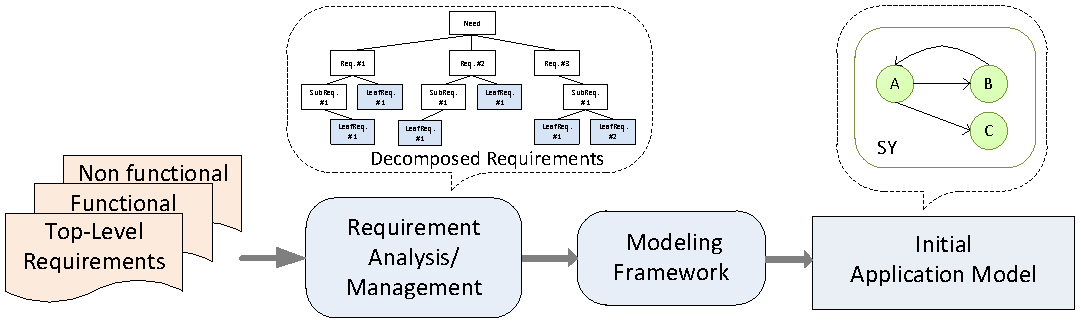
\includegraphics[width=\linewidth]{figs-src/specification.pdf}
	\caption{Specification phase of the proposed methodology.}
	\label{specification}
\end{figure}

The operational flow of the proposed transformation-based methodology is shown in Figure \ref{specification} and \ref{transformation} (in the following, words in \textit{italics} refer to the corresponding part in these figures). It comprises two main phases: 1) specification phase, and 2)  transformation phase, which belong to at least two  abstraction levels: the functional abstraction level and the functions decomposed to components abstraction level. The phases are elaborated and demonstrated by a running tutorial, but representative, example of a typical image processing application throughout this section. The goal is to show the use of our methodology and to explain the introduced concepts and techniques. 

%The operational flow of the proposed transformation-based methodology is shown in Figure \ref{specification} and \ref{transformation} (in the following, words written in \textit{italics} refers to the corresponding part in these figures). It comprises two main phases: 1) Specification phase, 2)  transformation phase, which belong to at least two  abstraction levels including the functional abstraction level and the functions decomposed to components abstraction level, respectively. The phases are elaborated in the following and are demonstrated by a running example of a typical image processing application throughout this section. The goal is to show the use of our methodology by this tutorial, but representative example and to explain the introduced concepts and techniques. 

\subsection{Specification Phase}
Figure \ref{specification} shows the specification phase of our transformational design flow. The starting point is requirement specification. The requirements that are usually in text format (\textit{Top-level Requirements}), are specified by means of an executable model. This step of design starts with breaking functional and non-functional requirements into several sub-requirements, so-called \textit{Decomposed Requirements}, and continues to  decompose them to smaller ones (\textit{Requirement Analysis/Management Tool})~\cite{grady2010system}. The result of this step is a requirements tree. It should be noted that the requirements will be further decomposed to be assigned to sub-systems, and the requirements tree will be extended and used for tracing decisions and their implications on other requirements during the transformation phase. At the next step of requirement specification, the leaf nodes of the requirement tree are associated with a set of functions by means of the chosen formal functional modeling framework (\textit{Modeling Tool}). These functions are arguments to the higher-order functions, i.e., process constructors and skeletons, and will not be touched and further refined during the transformation process. Therefore, the smaller the requirements in the leaf nodes of the requirements tree, the more opportunities for transformation in the transformation phase. The output of specification phase is an \textit{Initial Application Model} which at least specify all the functional requirements and is ready to be further refined in transformation phase of a design to include non-functional and implementation-dependent requirements, so-called \textit{Derived Requirements}, as well. Example \ref{ex:appModel} is an example of the specification model of the image processing application. 

\begin{figure}[t]
%    \captionsetup{position=b}
	\centering
	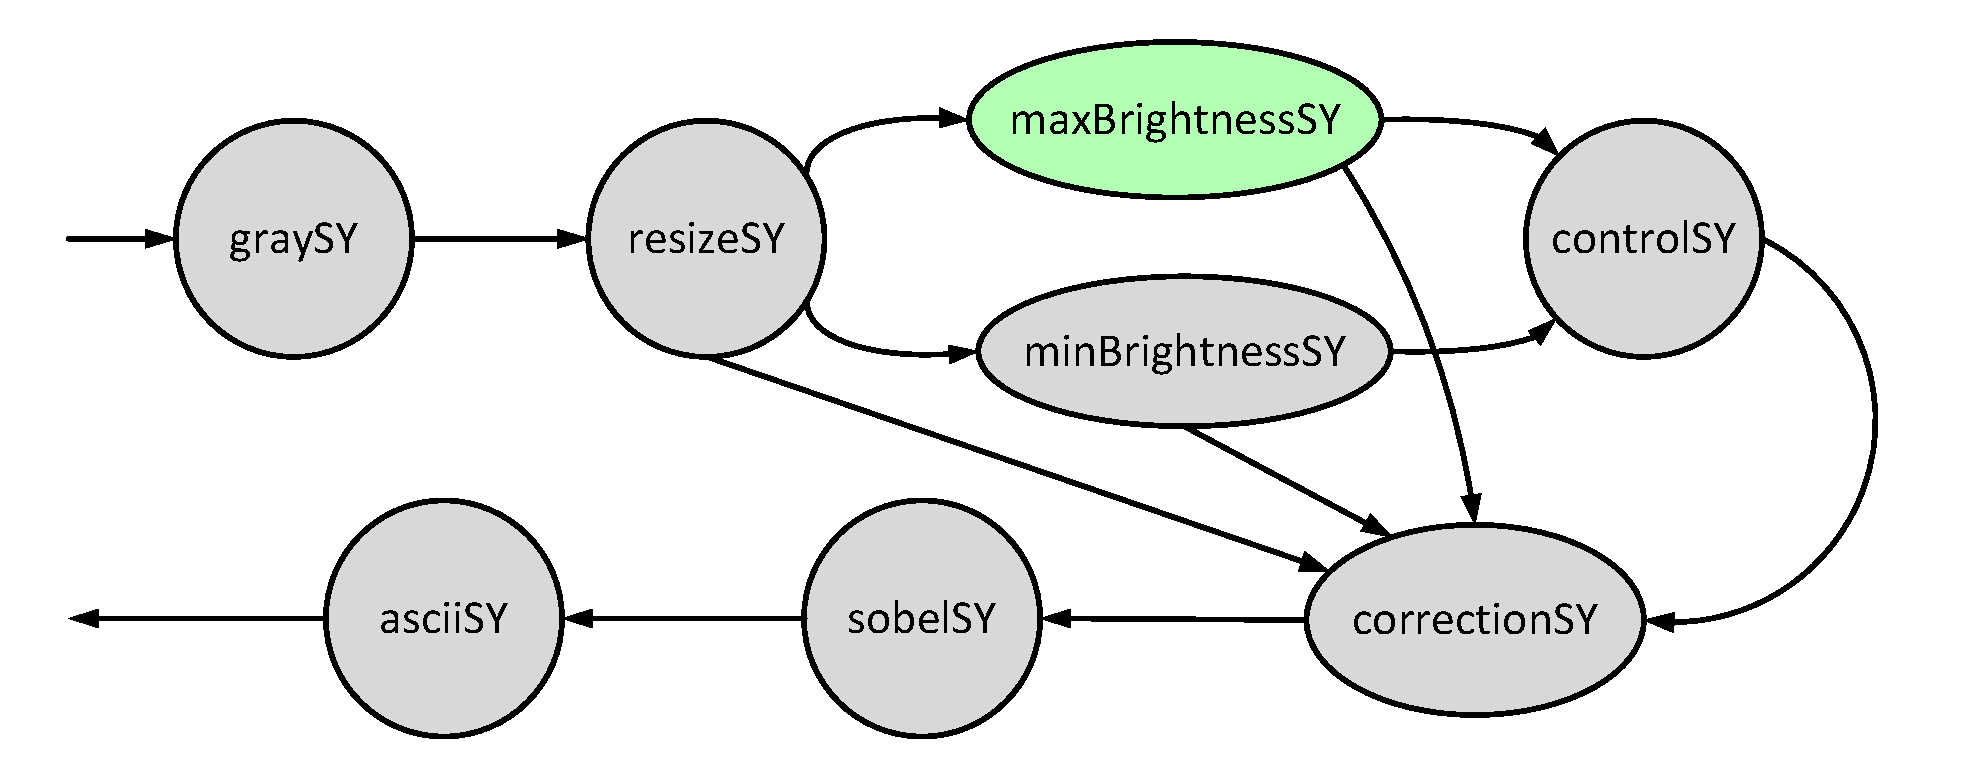
\includegraphics[width=2.3in]{figs-src/appModel.pdf}
	\caption{Image processing application model.}
	\label{appModel}
\end{figure}

\begin{exmp}\label{ex:appModel}
Figure \ref{appModel} illustrates the application model of an image processing application that converts an RGB-image to an ASCII art image, using brightness correction and edge detection (Sobel).
The application model is specified using ForSyDe \cite{sander2004system}, which has the features discussed in Section \ref{sec:application model}. It is based on the synchronous MoC and skeletons. 
In the synchronous MoC, a signal $s$ is modeled as a sequence of events, where each event $e_i$ has a tag and a value: $s = \{e_0, e_1, \dots\}$. The tag is implicitly given by the position of the event in the signal. A vector $v$ of $m$ elements is denoted by $v = [v_0, v_1, \dots, v_{m-1}]$. The process constructor $\mathit{mapSY}$ applies a function $f$ on each event of a signal, $\mathit{mapSY} (f, \{e_0, e_1, \dots\}) =  \{f(e_0), f(e_1), \dots\}$. The process constructor $\mathit{zipWithSY}$ applies a two-input function $f$ pairwise on two signals. The skeleton $\mathit{mapV}$ applies a function $f$ on each element of a vector,  $\mathit{mapV} (f, [v_0, v_1, \dots\, v_{m-1}]) =  [f(v_0), f(v_1), \dots, f (v_{m-1})]$. The skeleton $\mathit{reduceV}$ reduces a vector to a single value via an two-input function, $\mathit{reduceV} (f, [v_0, v_1, \dots\, v_{m-1}]) = f(v_0, f(v_1, f(\dots f(v_{m-2}, v_{m-1}))))$. The function $\mathit{unzipxSY}$ converts a signal of vectors to a vector of signals, while the function $\mathit{zipxSY}$ converts a vector of signals into a signal of vectors. These notations are used in the following examples.
We focus on \texttt{maxBrightnessSY} process. The executable code of the application model will be available at GitHub \cite{omitted}. 
\qed
\end{exmp}

\subsection{Transformation Phase}
\begin{figure}[t]
%    \captionsetup{position=b}
	\centering
	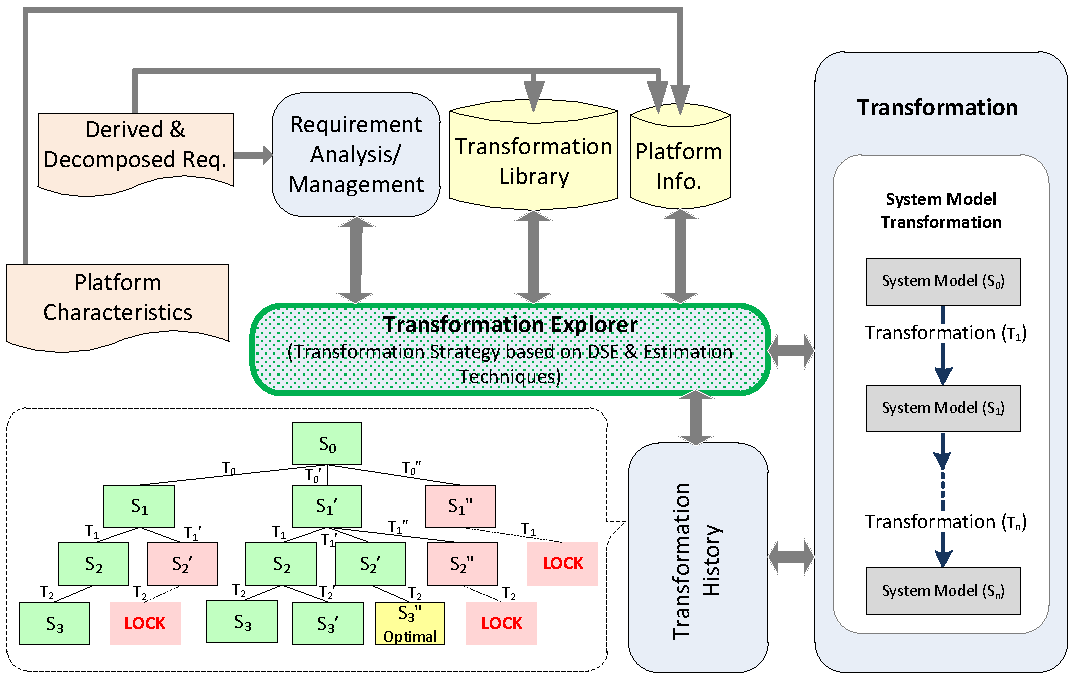
\includegraphics[width=\linewidth]{transformation.pdf}
	\caption{Transformation phase of the proposed methodology.}
	\label{transformation}
\end{figure}

Figure \ref{transformation} illustrates the transformation phase. Apart from derived requirements, another input to the design process are the \textit{Platform Characteristics}, i.e., the reuse of previously used architectures, design rules, guidelines and best practices.
Platform information including processors, memories and interconnection links that are allowed to be used during the platform transformation process are extracted from given platform characteristics. 
This phase mainly focuses on transforming the initial system model (\textit{System Model Transformation}) successively to several intermediate models (\textit{Transformation}).
Transformations are comprised of three steps: 1) pattern recognition: detecting possible transformations, 2) transform: transforming the system model by applying the corresponding transformation rule, and 3) efficient sequence  of  transformations: selecting the most promising sequence  of  transformations by virtue of DSE. The steps are elaborated and exemplified in the following. 

\begin{figure}[t]
%    \captionsetup{position=b}
	\centering
	\includegraphics[width=1.8in]{figs-src/MapMerge.png}
	\caption{The transformation rule ``MapMerge" \cite{sander2003system}.}
	\label{MapMerge}
\end{figure}
\begin{figure*}[t]
	\centering
	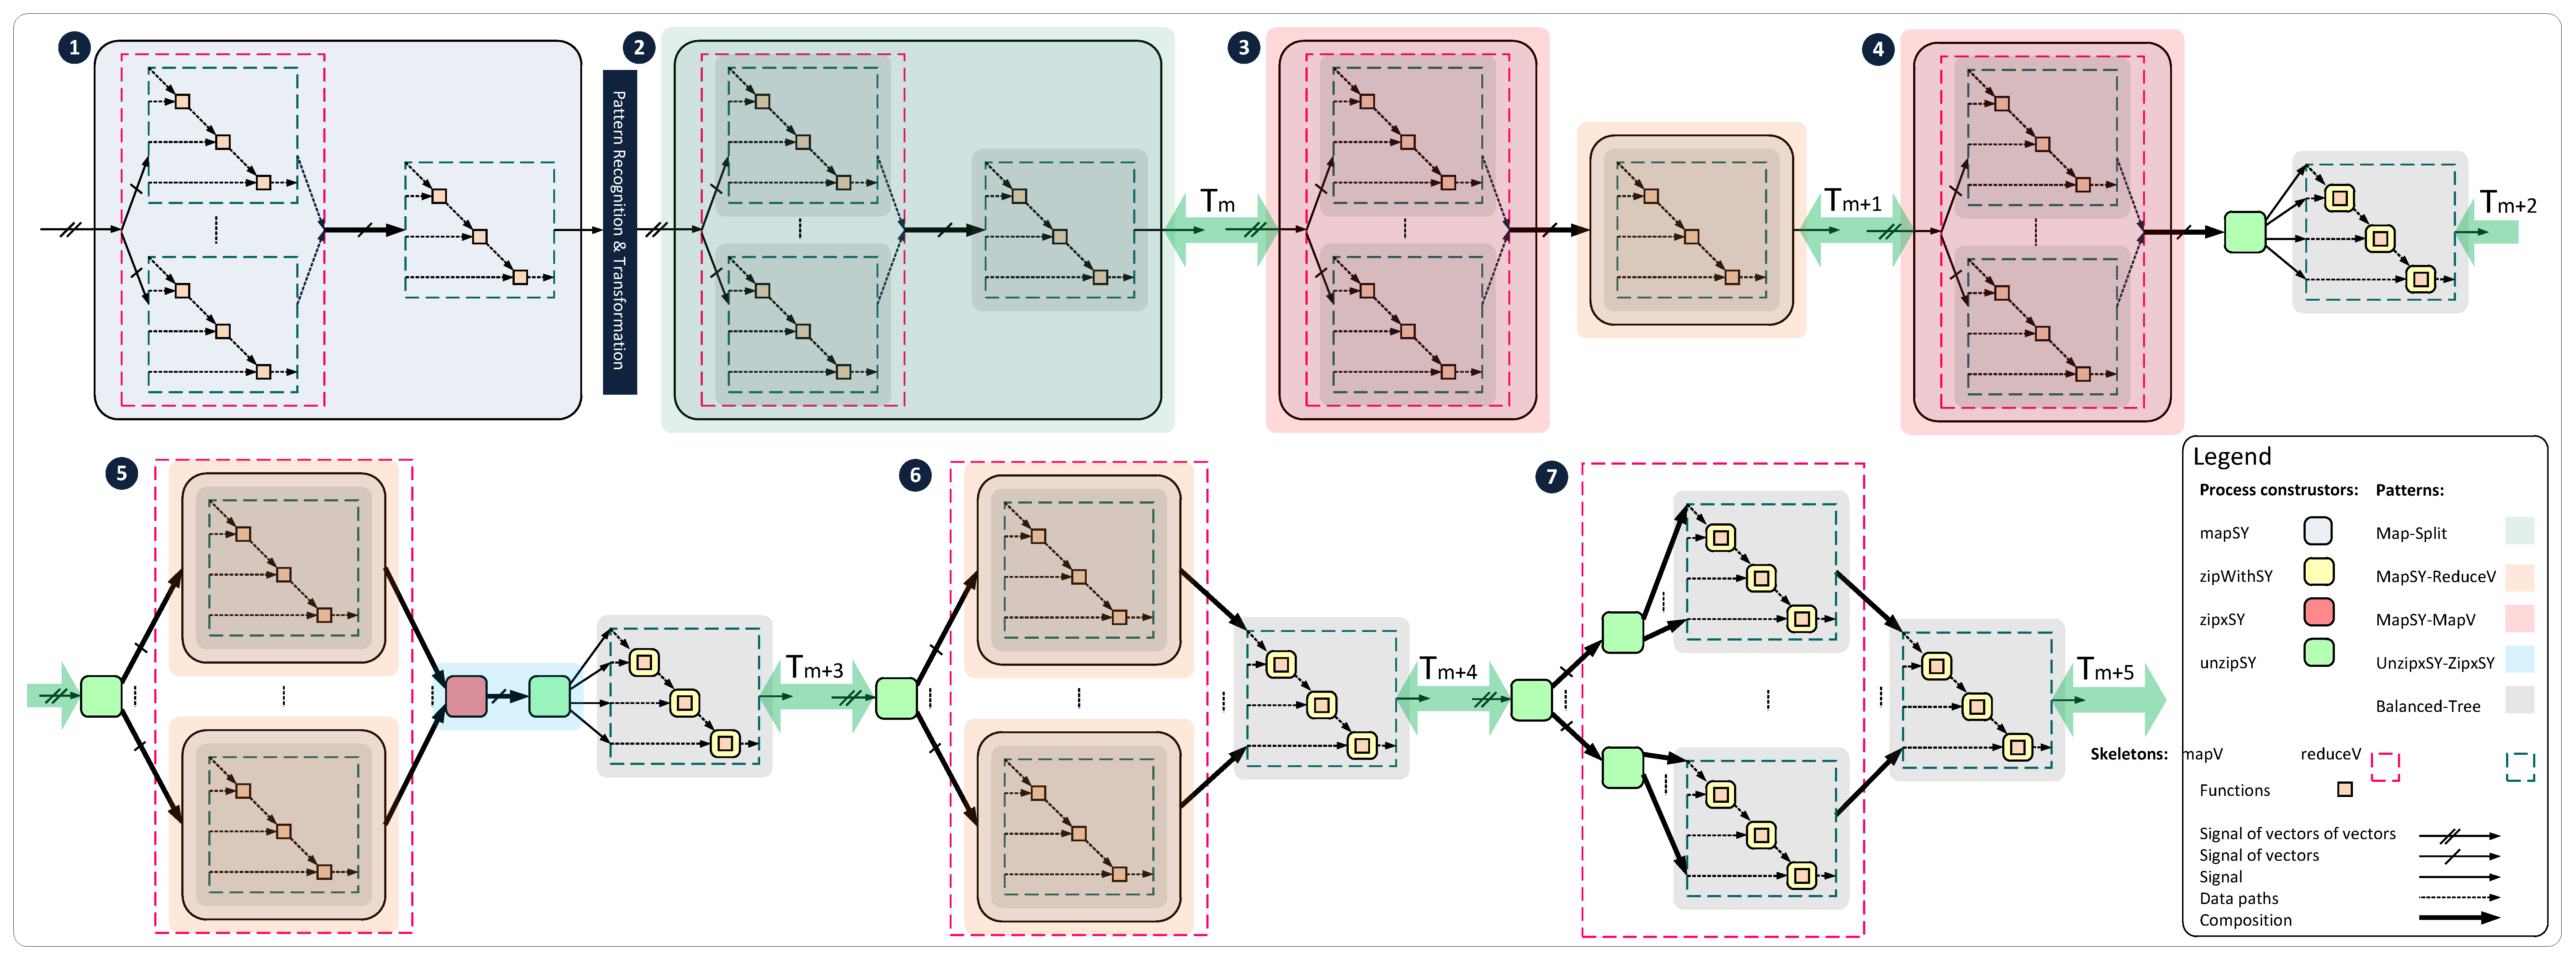
\includegraphics[width=\linewidth]{figs-src/brightness-transformation-flat.pdf}
	\caption{The transformation steps of maxBrightnessSY function.}
	\label{pattern}
\end{figure*}

\subsubsection{Pattern recognition}  
Since the proposed methodology is a rule-based transformational design method, the detection process of possible transformations is done using the patterns predefined in transformation rules. 

\begin{exmp}\label{ex:transformationRule}
As an example of transformation rules of application models, the transformation rule ``MapMerge" from~\cite{sander2003system} is shown in Figure \ref{MapMerge}. This transformation merges two processes. The ``Original Process Networks'' defines the pattern. The ``Transformed Process Network" describes how to transform the original process network.\qed
\end{exmp}

In Figure \ref{transformation}, an envisioned tool \textit{Transformation Explorer} fetches the patterns from \textit{Transformation Library}, explores the application model, and searches for the patterns. 
%It would be well advised to use a graph representation of the models undergoing transformations to be used for pattern recognition and to capture transformation results, as it is easier to transform from/into a graph. 
Defining the platform model-related transformations and enriching the transformation library are beyond the scope of this work and are deferred to future work. 
%In this work we only show how to conduct system developments using our integrated transformation-based methodology.

\begin{exmp}\label{maxBrightness}
Figure \ref{pattern} visualizes the pattern detection and transformation flow in transformation steps $T_m$ to $T_{m+4}$ of the process \texttt{maxBrightnessSY} (Example \ref{ex:appModel}). Patterns are shown by means of transparent colored boxes. The ForSyDe code, implemented in Haskell, of the transformation rules, including the original (patterns) and the transformed processes, used in this paper is given in Listing \ref{transformationRules}. In the following, the rules are  briefly explained.  
\begin{lstlisting}[float,floatplacement=H, language=Haskell, label={transformationRules}, caption= Haskell code of the transformation rules used in this paper.]
-- Transformation rules
-- Original Process = Transformed Process
---------------------------------------------------
-- Transformation Map-Split
mapSY (f . g) = mapSY f . mapSY g
-- Transformation MapSY-ReduceV
mapSY (reduceV f) = reduceV (zipWithSY f) . unzipxSY
-- Transformation MapSY-MapV
mapSY (mapV f) = zipxSY . mapV (mapSY f) . unzipxSY
-- Transformation ZipxSY-UnzipxSY
zipxSY . unzipxSY = id
-- Transformation Balanced-Tree
reduceV f vs = reduceTreeV f vs
reduceTreeV _ (a:>NullV) = a -- single element
reduceTreeV f vs =  -- tree stages recursion
  reduceTreeV f (mapV (reduceV f) (groupV 2 vs))
-- Transformation Serialize-Clock-Domain
delaySY s0 . mapSY (reduceV f)  vs =
downDI (length vs) . mooreSY (f) (id) s0 . par2serxDI
\end{lstlisting}

\begin{itemize}[leftmargin=*]
	\setlength{\parskip}{1pt} 
	\setlength{\itemsep}{0pt plus 0pt}
    \item \texttt{Map-Split}: This rule is the reverse transformation rule of the rule MapMerge (Figure \ref{MapMerge}), and is based on the identity \texttt{mapSY (f . g) = mapSY f . mapSY g} \cite{sander2004system}.
    \item \texttt{MapSY-ReduceV}: Since the ForSyDe compilation rules treat a process as a single entity during synthesis and does not divide a process further, this rule is used to convert a process that includes potential data parallelism, i.e., \texttt{reduceV}, into a parallel process network with the same function.
    \item \texttt{MapSY-MapV}: This rule provides the same benefit as the  rule \texttt{MapSY-ReduceV} does. 
    \item \texttt{ZipxSY-UnzipxSY}: This rule is based on the identity \texttt{zipxSY . unzipxSY = id}, and increases the level of parallelism.
    \item \texttt{Balanced-Tree}: This rule transforms a combinational process to a balanced one. It can be used if the input function is combinational and its operator is associative \cite{sander2004system}.
    \item \texttt{Serialize-Clock-Domain}: This rule \textquote{transforms a combinatorial processes of a regular structure into a structure with two clock domains that uses an FSM process to schedule the operations into several clock cycles} \cite{sander2004system}.
\end{itemize}
Step \circled{1} of Figure \ref{pattern} shows the original process  \texttt{maxBrightnessSY}. Pattern recognition and transformation starts from Step \circled{2}. 
%In the original process network two patterns, related to  transformation rules \texttt{Map-Split} and \texttt{Balanced-Tree} are detected (\circled{2}) and in transformation $T_m$, transformation rule \texttt{Map-Split} is applied, and the transformed process network is illustrated in Step \circled{3}. 
Table \ref{patterndetection} summarizes detected patterns and applied transformations in each step of Figure \ref{pattern}. \qed
\begin{table*}[t]
    \centering
    \caption{Pattern recognition and transformation steps of Figure \ref{pattern}.}
    \begin{tabular}{c||c|c|c}
        \hline
        \textbf{Transformation step} & \textbf{Detected patterns} & \textbf{Selected transformation} & \textbf{Applied transformation} \\
        \hline
        \circled{2} & \texttt{Balanced-Tree}, \texttt{Map-Split} & \texttt{Map-Split} & \circled{2} $\xrightarrow[]{T_m}$ \circled{3}\\
        \hline
        \circled{3} & \texttt{Balanced-Tree}, \texttt{MapSY-MapV}, \texttt{MapSY-ReduceV} & \texttt{MapSY-ReduceV} & \circled{3} $\xrightarrow[]{T_{m+1}}$ \circled{4}\\
        \hline
        \circled{4} & \texttt{Balanced-Tree}, \texttt{MapSY-MapV} & \texttt{MapSY-MapV} & \circled{4} $\xrightarrow[]{T_{m+2}}$ \circled{5}\\
        \hline
        \circled{5} & \texttt{Balanced-Tree}, \texttt{MapSY-ReduceV}, \texttt{ZipxSY-UnzipxSY} & \texttt{ZipxSY-UnzipxSY} & \circled{5} $\xrightarrow[]{T_{m+3}}$ \circled{6}\\
        \hline
        \circled{6} & \texttt{Balanced-Tree}, \texttt{MapSY-ReduceV} & \texttt{MapSY-ReduceV} & \circled{6} $\xrightarrow[]{T_{m+4}}$ \circled{7}\\
        \hline
        \circled{7} & \texttt{Balanced-Tree} & \texttt{Balanced-Tree} & \circled{7} $\xrightarrow[]{T_{m+5}}$ \circled{8}\\
        \hline
    \end{tabular}
    \label{patterndetection}
\end{table*} 
\end{exmp} 
\subsubsection{Transform}
Transformation rules define how to transform the system model. Transformation rules in conjunction with \textit{Transformation History} (Figure \ref{transformation}) provide  transparent transformations, as they enable transformations backward and forward. 
\begin{exmp}
Figure \ref{pattern} shows how the original process \texttt{maxBrightnessSY} is transformed to several intermediate models, using the formats defined as ``transformed process network" in rules. Moreover, Listing \ref{code} shows the transformation of its ForSyDe code. The ForSyDe code of the original image processing application (Figure \ref{appModel}) and that of the transformed application model will be available at GitHub \cite{omitted}.\qed
\begin{lstlisting}[float,floatplacement=H, language=Haskell, label={code}, caption= The transformation of process maxBrightnessSY.]
maxBrightness = mapSY (reduceV f . mapV (reduceV f))
-- Transformation Map-Split
maxBrightness = mapSY (reduceV f) . mapSY (mapV (reduceV f))
-- Transformation MapSY-ReduceV
maxBrightness = reduceV (zipWithSY f) . unzipxSY . mapSY (mapV (reduceV f))
-- Transformation MapSY-mapV
maxBrightness = reduceV (zipWithSY f) . unzipxSY . zipxSY . mapV (mapSY (reduceV f)) . unzipxSY
-- Transformation ZipxSY-UnzipxSY
maxBrightness = reduceV (zipWithSY f) . mapV (mapSY (reduceV f)) . unzipxSY
-- Transformation MapSY-ReduceV
maxBrightness = reduceV (zipWithSY f) . mapV (reduceV (zipWithSY f) . unzipxSY) . unzipxSY
\end{lstlisting}
\end{exmp}
\begin{table*}[t]
    \centering
    \caption{Part of the transformation tree of process maxBrightnessSY.}
    \begin{tabular}{c|c|c}
        \hline
        \multicolumn{3}{c}{\makecell{\textbf{Original system model:} $S_n = (R_i, A_j, M_k, P_l)$, $A_j:reduceV (mapSY f)$, $R_i:t_{prop}\leq60$}}\\
        \hline
        \textbf{Sequence 1} & \textbf{Sequence 2} & \textbf{Sequence 3}\\
        \hline
        \hline
        -&-&\makecell{$S_n = (R_i, A_j, M_k, P_l)$\\$A_j \xrightarrow[]{MapSY-ReduceV} A_{j+1}$}\\
        \hline
        \makecell{$S_n = (R_i, A_j, M_k, P_l)$\\$A_j \xrightarrow[]{Balanced-Tree} A_{j+1}$}&-&\makecell{$S_n = (R_i, A_{j+1}, M_k, P_l)$\\$A_{j+1} \xrightarrow[]{Serialize-Clock-Domain} A_{j+2}$} \\
        \hline
        \makecell{$S_n = (R_i, A_{j+1}, M_k, P_l)$\\$P_l \xrightarrow[]{HW} P_{l+1}$}& \makecell{$S_n = (R_i, A_{j}, M_k, P_l)$\\$P_l \xrightarrow[]{HW} P_{l+1}$}&
        \makecell{$S_n = (R_i, A_{j+2}, M_k, P_l)$\\$P_l \xrightarrow[]{SW} P_{l+1}$}\\
        \hline
        \makecell{$S_n = (R_i, A_{j+1}, M_k, P_{l+1})$\\$M_k \xrightarrow[]{A_{j+1},P_{l+1}} M_{k+1}$} & \makecell{$S_n = (R_i, A_{j}, M_k, P_{l+1})$\\$M_k \xrightarrow[]{A_{j},P_{l+1}} M_{k+1}$} &
        \makecell{$S_n = (R_i, A_{j+2}, M_k, P_{l+1})$\\$M_k \xrightarrow[]{A_{j+2},P_{l+1}} M_{k+1}$}\\
        \hline
        \makecell{$S_n = (R_i, A_{j+1}, M_{k+1}, P_{l+1})$\\$R_i \xrightarrow[]{decompose} R_{i+1}:2*t_t\leq60$} & \makecell{$S_n = (R_i, A_{j}, M_{k+1}, P_{l+1})$\\$R_i \xrightarrow[]{decompose} R_{i+1}:3*t_t\leq60$}&
        \makecell{$S_n = (R_i, A_{j+2}, M_{k+1}, P_{l+1})$\\$R_i \xrightarrow[]{decompose} R_{i+1}:t_{C-Code}\leq 60$}\\
        \hline
        \makecell{$S_n = (R_{i+1}, A_{j+1}, M_{k+1}, P_{l+1})$}& \makecell{$S_n = (R_{i+1}, A_{j}, M_{k+1}, P_{l+1})$}&
        \makecell{$S_n = (R_{i+1}, A_{j+2}, M_{k+1}, P_{l+1})$}\\
        \hline
    \end{tabular}
    \label{sequenceTran}
\end{table*} 
\begin{figure*}[t]
	\centering
	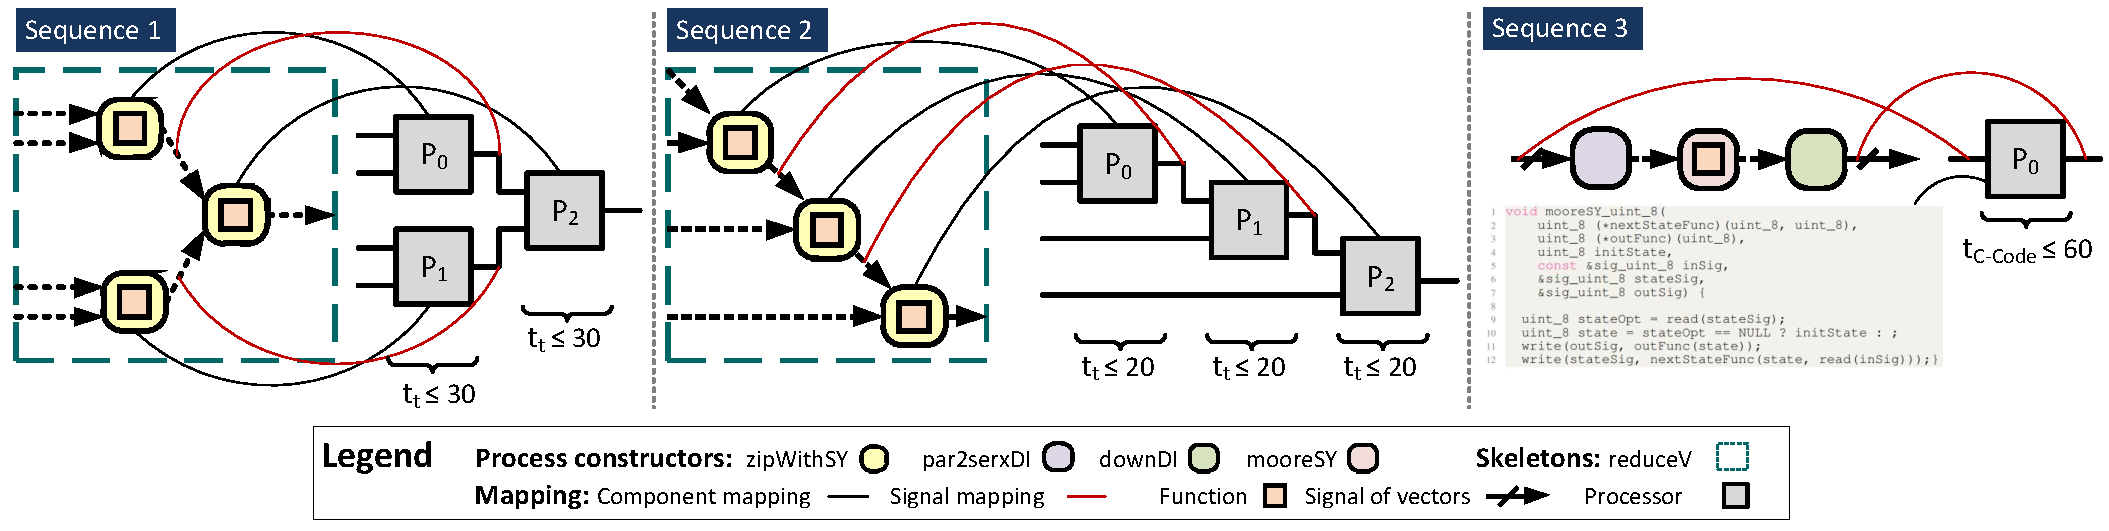
\includegraphics[width=0.986\linewidth]{figs-src/diffSequences.pdf}
	\caption{System models resulted from different sequences of transformations shown in Table \ref{sequenceTran}.}
	\label{sequenceResults}
\end{figure*}
%Exploration: We explore numerous design alternatives to find one that best satisfies ourconstraints. To do this, we  transform the initial de- scription into one moresuitable for implementation. We allocate a set of  system components and specify their  physical and performance constraints, as in  the example in Figure 2, where we allocated three memories, two ASICs, one proces- sor, and several buses. We partition the functional specification among allocated components. For guidance in these exploration subproblems, we estimate each alternative design’s quality \cite{gajski1995specification}.
%In this phase there is no WCETs for the tasks. WCETs come in the mapping model in Phase B.%PIM: list of functions

\subsubsection{Efficient sequence  of  transformations}
In Table \ref{patterndetection}, in Steps~\circled{2} to \circled{6}, there is always more than one possible transformation. The applied sequence of  transformations highly affects the implementation. Transforming different parts of the system model provides the opportunity to explore a large number of design alternatives and to achieve an efficient implementation. As a guideline in exploring these sub-problems, we take advantage of early stage DSE, at the higher abstraction levels where there is no detailed knowledge about the implementation platform, and traditional DSE techniques \cite{pimentel2016exploring}, at the lower levels.
\begin{exmp}
Table \ref{sequenceTran} shows part of the transformation tree of process \texttt{maxBrightnessSY}, i.e., \texttt{reduceV~(mapSY f)}, as three different sequences of transformations, and Figure~\ref{sequenceResults} illustrates the system model resulting from each of them.
For each sequence of transformations, Table~\ref{sequenceTran} shows how the original system model, represented in the RAMP-format, is transformed by a step-wise application of transformation rules. 
In sequence 1, the transformation rule \texttt{Balanced-Tree} is used and a hardware implementation is preferred. However, in sequence 2,  a hardware implementation of the original application model is selected. Finally, in sequence 3, after transformation \texttt{Serialize-Clock-Domain} (Listing \ref{transformationRules}), the application model includes the process \texttt{mooresy (max) (id) 0} constructed by process constructor \texttt{mooreSY}, which is interpreted as a FSM \cite{sander2004system}. The software implementation (C-code) of the application model is mapped to a single core. Figure \ref{sequenceResults} also shows the transformations of requirements, where the top-level requirement $R_i:t_{prop}\leq60$ has been transformed into derived requirements on the individual sub-systems. 

In this step, DSE techniques are used to estimate the quality of each implementation and define the most promising one. \qed
%For the platform model, annotated components from the component library are used. 
\end{exmp}




%\begin{itemize}
%    \item Initial platform:
%    \begin{itemize}
%        \item @SAAB: Initial platform is needed (memory, bandwidth, ...).
%        \item @Ingo: Initial platform is an empty platform.
%        \item @Fahimeh: one single node.
%    \end{itemize}
%    \item The initial contract $C_0$: formal specification of requirements.
%\end{itemize}


%Phase B mainly focus on transforming the initial models of the application, platform, mapping, and refined requirements (\textit{System Model transformation})  successively to several intermediate models (\textit{Transformation}). Transformations are comprised of three steps: 1) detecting possible transformations, 2) selecting one of them to be applied in the next transformation step, 3) refining the system model. 
%We propose a transformation strategy for the first and second task and a rule-based transformation approach for the third one as follows:

%\begin{itemize}
% \item \textbf{Transformation strategy:}
% The detection process of possible transformations is done by means of the paterns pre-identified by the transformation rules. Moreover, the refinemnts of both the application model and the platform model follow the composition rules defined by the underlying modeling framework. In other owrds, the initial application model fed into Phase B is a process network, i.e., a functional composition of processes. 
% For  such application models that are based on the features defined in Section \ref{sec:application model}, process constructors identify applicable composition patterns. Also, platform models, supporting compositional transformation, follow the composition rules stored in the \textit{Platform Information} library, as well as defining some notations of dominance to help for detecting pareto-compositinal transformations of the components. It would be well advised to use a graph representation of the models undergoing transformations to capture transformation results as it is easier to transform from/into a graph. To detect the possible transformations, Transformation Explorer explores the graph representation of the system model and search for the patterns. 

 
%The transformation tree shown in Phase B of Figure \ref{Sequence} illustrates the complexity of the first two steps of each transformation. It is the transformation tree of a transformation library including only three transformation rules, i.e., $\{T, T', T''\}$. In the first transformation step, transformations $T_0$ and $T'_0$ are possible. It is possible to either try both of them out or to select the transformation that is dominant in the current transformation step.  The first strategy is a comprehensive solution that leads to an optimal solution, while the second one ensures at least a \textit{good enough} solution that can be the optimal solution, as well. The proposed transformation strategy follows the second strategy and select one of the possible transformations by virtue of a \textit{Transformation Explorer} to transform the system model in a timely manner. The transformation explorer first filters the transformations that do not satisfy requirements out and then takes advantage of \textit{Refined Requirements}, \textit{Early-stage DSE}, and \textit{Estimation Techniques} to find the pareto-refinemnt. 


  
 %\item \textbf{transformation:}
% TRANSFORM is a rule-based transformation methodology. The rules define the formats of the original  (patterns) and refined process networks as well as the implication of the design transformation. The implications pave the way for verifying the transformations. It is also worth mentioning that the transformation rules filling the transformation library are highly dependent on the application domain. A clear understanding of the underlying application domain is extremely important and necessary to design suitable transformation rules.  
%\end{itemize}

 
 

%For example, given an in-termediate result represented in ETPN, an algorithm can be used to estimate its implementation cost, checkwhether that satisfies the design constraints, and automatically choose a transformation to apply to the de-sign which produces another intermediate result with improved cost. ETPN, for example, is used by theCAMAD hardware synthesis system [Pen 88b] to support an iterative transformation approach to carry outthe synthesis tasks. CAMAD first generates a preliminary (default) design in ETPN format from the inputspecification. It then applies transformations one by one to the preliminary result so as to obtain better so-lutions. This iterative process is finished when satisfactory results have been reached. The data path is thentransformed  into  a  net-list  and  the  control  Petri  net  into  a  microprogram.  The  proposed  silicon/softwarecompiler environment will use the same strategy \cite{peng1991unified}.
%Synthesis can further besplit into 1) decision making, which is theeducated(i.e. anaylsis-based) process ofsteering the design flow; and 2) transformation, which is the task of incorporating thesedecision into the behavioral model, resulting into an implementation model.


%very important: learning
%Product design decisions based on performance needs
%Dependencies between requirements must be tracked.
%Keeping history of transformations: The  design  process  and  design  decisions  are documented,   thus   the   whole   process   is repeatable \cite{wu2001transformational}.
%In particular, a design methodology should separate:1) function (what the system is supposed to do) from architecture (how it does it) and 2) communication from computation \cite{sander2004system}.
%based on the platform characteristics and platform info., the expected worst case execution time of each task on each processing element can be calculated. 
%when there are dual-criticality tasks, at least three nodes are needed.
%transform heavily relays on design rules. Design rules also speed up DSE.
%\subsection{Phase C}

% $mapV (mapSY f)$ should be mapped on GPU (since it is a stream processing 

%Accelerator: For      example,      in      HW/SW      co-design,transformation  techniques  can  be  employed  inthe system's custom parts that are not covered bypre-designed building blocks (IPs).

%The last paragraph: Of course, there are still difficulties in applying apurely transformational approach to large systemdesign.   However,   the   incorporation   of   thisapproach  into  the  design  methodology  will  offerthe  opportunities  to  improve  the  design  process \cite{wu2001transformational}.

%should the figure be changed to include mapping and design constraint transformations as well?


%\begin{lstlisting}[float,floatplacement=H, language=C++, label={code}, caption= The transformation of process maxBrightnessSY.]
%void mooreSY_uint_8(
%    uint_8 (*nextStateFunc)(uint_8, uint_8),
%    uint_8 (*outFunc)(uint_8),
%    uint_8 initState,
%    const &sig_uint_8 inSig,
%    &sig_uint_8 stateSig,
%    &sig_uint_8 outSig) {

%  uint_8 stateOpt = read(stateSig);
%  uint_8 state = stateOpt == NULL ? initState : ;
%  write(outSig, outFunc(state));
%  write(stateSig, nextStateFunc(state, read(inSig)));}
%\end{lstlisting}


%%% Local Variables:
%%% mode: latex
%%% TeX-master: "../paper"
%%% End: